\def\year{2015}
%File: formatting-instruction.tex
\documentclass[letterpaper]{article}
\usepackage{aaai}
\usepackage{times}
\usepackage{helvet}
\usepackage{courier}
\frenchspacing
\setlength{\pdfpagewidth}{8.5in}
\setlength{\pdfpageheight}{11in}
\pdfinfo{
/Title (Insert Your Title Here)
Matheus Redecker (Put All Your Authors Here, Separated by Commas)}
\setcounter{secnumdepth}{0}  

\usepackage[portuguese]{babel}
\usepackage[utf8]{inputenc}
\usepackage{graphicx,url}

 \begin{document}
 \nocopyright
% The file aaai.sty is the style file for AAAI Press 
% proceedings, working notes, and technical reports.
%
\title{ Domínio das Pranchas }
\author{Matheus Redecker\\
Pontifícia Universidade Católica do Rio Grande do Sul - PUCRS\\
Av. Ipiranga, 6681 \\
Porto Alegre, Rio Grande do Sul\\
}
\maketitle

\section{Introdução}
Neste artigo será demonstrado uma alternativa de solução para o domínio das pranchas. Esse domínio pode ser descrito como um conjunto de ilhas pequenas onde apenas um agente pode estar em cima. As ilhas podem ter uma ligação com outras por meio de uma prancha, mas para isso acontecer elas devem ser adjacentes. Os agentes devem se mover pelas ilhas por meio das pranchas, então será necessário que o agente troque as pranchas de lugar para criar ligações entre ilhas que inicialmente não estão conectadas. O domínio apresenta três ações que podem ser executadas para atingir os objetivos, a ação de atravessar de uma ilha para outra, para isso acontecer deve ter uma prancha ligando as duas ilhas, a ação de pegar uma prancha, onde o agente pega a prancha que faz conexão com a ilha que ele está em cima e segura para si, cada agente pode segurar apenas uma prancha, e a ação de colocar a prancha entre duas ilhas, assim fazendo a ilha ser acessível. 

Na próxima seção será apresentado a formalização utilizada para a representação deste domínio, separando por problemas simples e problemas mais complexos, junto com uma seção que irá mostrar os predicados usados e como as ações para resolver o problema foram construídas, contudo não será apresentado nenhuma implementação direta dos problemas, pois com as explicações contidas no artigo dão subsidio para a construção da solução utilizando a formalização e ainda será apresentado uma seção de conclusão que mostra como foi a experiência e os problemas encontrados na realização deste trabalho.

\section{Formalização do Dominio}
Esta seção apresenta a formalização do domínio começando de problemas simples e avançando até problemas mais complexos, sendo assim a explicação será dividia em duas partes, uma para problemas mais simples servindo de compreensão do que deve ser feito, e uma seção que apresenta problemas mais avançados que exigem a compreensão do funcionamento das ações. Com os problemas descritos serão apresentados uma alternativa de como esses problemas foram resolvidos.

\subsection{Problemas Simples}
Para compreender o funcionamento das ações dois problemas foram criados para demonstrar o que cada ação deve realizar. O primeiro problema é dado para a codificação da primeira ação, a de um agente atravessar de uma ilha para outra, o arquipélago tem duas ilha ligadas por uma prancha, o agente começa em uma delas e tem como objetivo atravessar para a outra ilha. Já o segundo problema tem como objetivo a utilização das outras duas ações, assim o arquipélago tem três ilhas em sequencia, o agente começa na ilha central e cada lado contem uma outra ilha, a ilha uma das ilhas tem ligação com a sua por meio de uma prancha, o objetivo é trocar a prancha de lugar e fazer com que a outra ilha tenha acesso a sua. 

\subsection{Problemas Avançados}
Depois dos problemas simples terem sido codificados, é possível fazer problemas que tenham mais movimentos e que não sejam apenas teste das ações, ou seja, fazer com que as ações sejam realizadas de forma cooperativa. Para isso então o primeiro problema dessa classe é representado por um arquipélago com três ilhas em sequencia, o agente está em uma ilha do canto existe uma ponte que liga a ilha do agente com a ilha central, e o objetivo é cruzar as ilhas até a ilha no outro extremo. Para isso a gente vai precisar atravessar e mudar a prancha de lugar. Já o outro problema é composto por dois agentes e um arquipélago de quatro ilhas três delas em sequencia e ultima delas para o norte da ilha central, dessas quatro ilhas 3 delas estão ligadas, a ilha central tem ligação com uma das ilhas do seu lado e com a ilha ao norte, um dos agentes está isolado, e o objetivo é que os agentes fiquem a uma ilha de distancia. 

\section{Experimentos}

Para representar as ações foi necessário criar predicados que representam os estados dos agentes e também do ambiente, para isso foram criados cinco predicados que estão demonstrados a seguir.

 \begin{verbatim}
    (on ?agent ?island)
    (clear ?island)
    (plankAt ?plank ?island1 ?island2)
    (have ?agent ?plank)
    (side ?island1 ?island2)
\end{verbatim}

%explicar cada um dos predicados e falar porque a escolha de cada um deles
Esses predicados foram utilizados pelo fato de que essa possibilidade de solução é preciso um predicado para dizer em qual ilha o agente está situado(on), um predicado que denota que uma ilha não tem nenhum agente em cima(clear), outro predicado para mostrar que existe uma prancha entre duas ilhas plankAt, um predicado para denotar que o agente está segurando uma prancha(have) e para os problemas avançados foi necessário um predicado para denotar a adjacência das ilhas(side).

Utilizando os predicados apresentados acima foi construído as três ações citadas nas seções anteriores. A descrição de cada ação junto com o cabeçalho da ação em pddl, está abaixo.

A ação de atravessar de uma ilha para outra é denominada cross. Para que ela aconteça é necessário que o agente esteja em uma ilha que a ligação de uma prancha com a ilha que ele deseja alcançar e que a ilha esteja livre, se isso for satisfeito o agente passa para aquela ilha e sinaliza que está na ilha nova, que ilha não está mais livre e que a sua antiga ilha passou a ficar livre. 

\begin{verbatim}  
    (:action cross
    :parameters (?island1 ?island2
                 ?agent1  ?plank)
    )
\end{verbatim}

Para pegar uma prancha a ação que representa é a ação chamada pick. Para que ela aconteça o agente não pode estar com nenhuma outra prancha e ainda estar em uma ilha que tenha conexão com outra ilha por meio de uma prancha. Se isso for satisfeito o agente passa a ter uma prancha e a ação sinaliza que agora não há mais uma prancha entre aquelas ilhas. 
\begin{verbatim}  
    (:action pick
    :parameters (?island1 ?island2
                 ?agent1 ?plank)
    )
\end{verbatim}

Depois do agente conseguir pegar a prancha é necessário que ele a coloque entre duas ilhas, a ação que representa essa função é chamada de lay, para ela ser executada é necessário que não tenha uma prancha entre essas ilhas, que o agente segure uma prancha e que elas sejam adjacentes uma a outra. Se isso acontecer o agente coloca sua prancha e a ação sinaliza para o ambiente que agora existe uma prancha que liga as duas ilhas. 
\begin{verbatim}  
    (:action lay
    :parameters (?island1 ?island2
                 ?agent1 ?plank)
    )
\end{verbatim}


%FALAR QUE EU TIVE QUE DObRAR OS PREDICADOS PARA ESPELHAR AS AÇÕES
Com a implementação feita um problema foi encontrado, quando os predicados plankAt ou o side tinham as ordens trocadas dos seus argumentos, ação certa não era encontrada, assim se fazendo necessário o duplicar os predicado com apenas a troca dos parâmetros. Como por exemplo:
 \begin{verbatim}
      (side ?island1 ?island2)
      (side ?island2 ?island1)
\end{verbatim}

Formalizando os problemas apresentados na seção anterior foi comparado seu desempenho mostrando a evolução do tempo de execução e também da memória utilizada para encontrar o plano correto, levando em consideração que o tamanho do plano correto para cada problema tem 1, 2, 4, 11 passos, dois gráficos estão apresentados para a comparação, na figura \ref{tempo} podemos ver que a medida que o problema fica mais complexo o tempo para atingir a solução cresce.  Já a memória utilizada para o problema é apresentada na figura \ref{memoria}, onde podemos ver que apenas no ultimo problema temos um crescimento muito alto. 

\begin{figure}[ht]
\centering
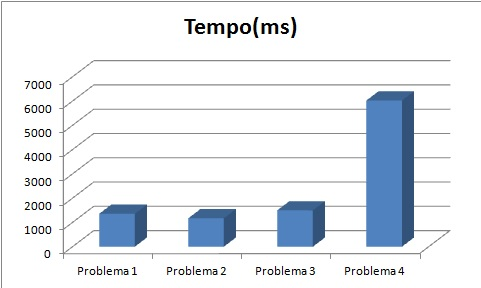
\includegraphics[scale=0.6]{tempo.jpg}
\caption{}
\label{tempo}
\end{figure}

\begin{figure}[ht]
\centering
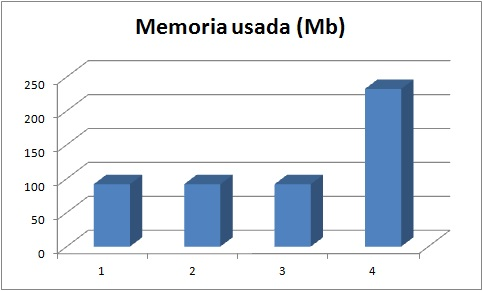
\includegraphics[scale=0.6]{memoria.jpg}
\caption{}
\label{memoria}
\end{figure}


\section{Conclusão}

\noindent 
A codificação dos problemas foi uma experiência nova e agradável, como os domínios e os problemas são especificados em lógica, que eu particularmente gosto, foi gratificante construir a solução para esse problema. 

Contudo minha alternativa de solução não foi a melhor possível, tive dificuldades de encontrar uma maneira mais limpa de apresentar os problemas. A duplicação de predicados se deu pelo fato de que não consegui representar o operador "ou" somente com operadores "e", sei que existe uma maneira de se fazer isso, o que eu encontrei para resolver esse problema foram as leis de Morgam, mas não tive sucesso na aplicação delas.

A utilização do JavaGP para a resolução dos problemas foi de fácil compreensão, a sintaxe utilizada é simples e o seu desempenho para esses problemas foi satisfatório.
% FALAR ALGUMA COISA DO JAVA GP DA SINTAXE DOS OPERADORES
\end{document}
